\documentclass[tikz,border=4pt]{standalone}
\usepackage{amsmath}
\usepackage{tikz}
\usetikzlibrary{arrows.meta,positioning,fit,backgrounds,calc,shapes.geometric,decorations.pathreplacing,patterns}
\usepackage{xcolor}
\renewcommand{\familydefault}{\sfdefault}
\definecolor{cdata}{HTML}{1F5FA8}
\definecolor{cctrl}{HTML}{15796F}
\definecolor{cres}{HTML}{6A4C93}
\definecolor{cgray}{HTML}{5A6570}
\definecolor{cwarn}{HTML}{B4561B}
\tikzset{
  base/.style={rounded corners=1.8pt, line width=0.6pt, align=center, font=\scriptsize, inner sep=3pt, minimum height=8mm, text=black!85},
  data/.style={base, draw=cdata, fill=cdata!9},
  ctrl/.style={base, draw=cctrl, fill=cctrl!9},
  res/.style={base, draw=cres, fill=cres!9},
  art/.style={base, draw=black!65, fill=black!7},
  ext/.style={base, draw=cgray, fill=white, dashed},
  gate/.style={font=\tiny\bfseries, text=cwarn, draw=cwarn, rounded corners=1pt, inner sep=1.6pt, fill=white, line width=0.5pt},
  arr/.style={-{Stealth[length=2.0mm,width=1.5mm]}, line width=0.6pt, draw=cgray!85!black},
  arr2/.style={{Stealth[length=2.0mm,width=1.5mm]}-{Stealth[length=2.0mm,width=1.5mm]}, line width=0.6pt, draw=cgray!85!black},
  darr/.style={-{Stealth[length=2.0mm,width=1.5mm]}, line width=0.6pt, dashed, draw=cgray!85!black},
  lbl/.style={font=\tiny, text=cgray!90!black, inner sep=1pt},
  band/.style={rounded corners=3pt, line width=0.7pt},
}
\newcommand{\dotsep}{\,$\cdot$\,}
\renewcommand{\tiny}{\fontsize{6}{7}\selectfont}

\begin{document}
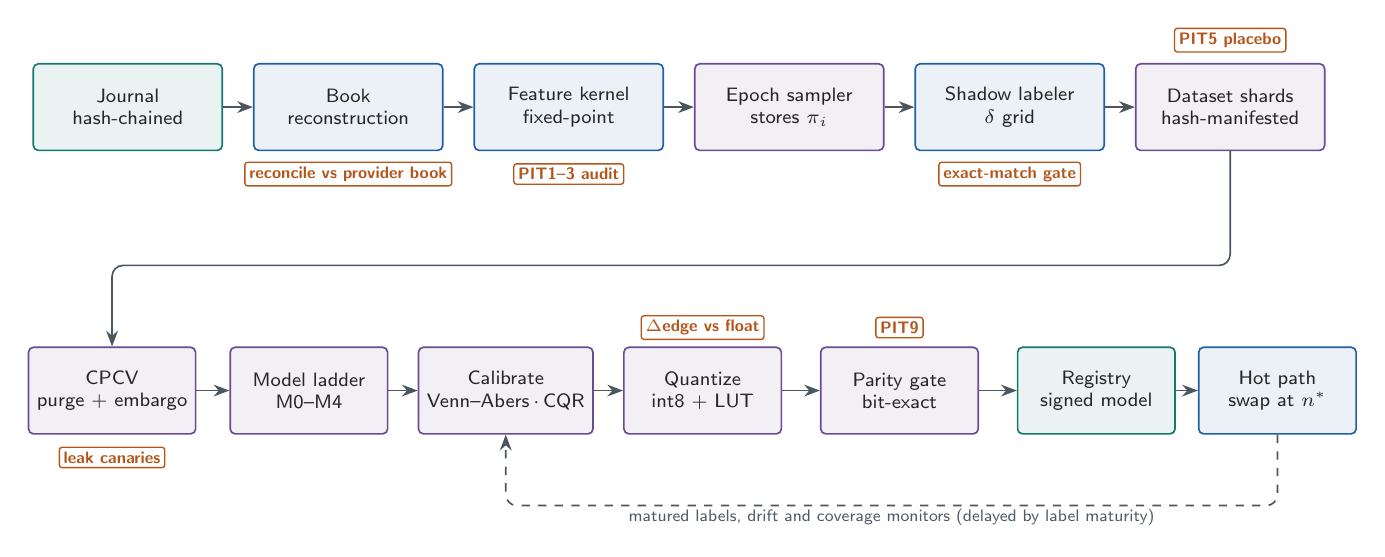
\begin{tikzpicture}
% row 1: data to dataset
\node[ctrl, minimum width=2.4cm, minimum height=11mm] (a1) at (1.4,6.0) {Journal\\hash-chained};
\node[data, minimum width=2.4cm, minimum height=11mm] (a2) at (4.2,6.0) {Book\\reconstruction};
\node[data, minimum width=2.4cm, minimum height=11mm] (a3) at (7.0,6.0) {Feature kernel\\fixed-point};
\node[res,  minimum width=2.4cm, minimum height=11mm] (a4) at (9.8,6.0) {Epoch sampler\\stores $\pi_i$};
\node[data, minimum width=2.4cm, minimum height=11mm] (a5) at (12.6,6.0) {Shadow labeler\\$\delta$ grid};
\node[res,  minimum width=2.4cm, minimum height=11mm] (a6) at (15.4,6.0) {Dataset shards\\hash-manifested};
\foreach \a/\b in {a1/a2,a2/a3,a3/a4,a4/a5,a5/a6}{\draw[arr] (\a) -- (\b);}
\node[gate] at (4.2,5.15) {reconcile vs provider book};
\node[gate] at (7.0,5.15) {PIT1--3 audit};
\node[gate] at (12.6,5.15) {exact-match gate};
\node[gate] at (15.4,6.85) {PIT5 placebo};
% row 2: training and release
\node[res,  minimum width=2.0cm, minimum height=11mm] (b1) at (1.2,2.4) {CPCV\\purge + embargo};
\node[res,  minimum width=2.0cm, minimum height=11mm] (b2) at (3.7,2.4) {Model ladder\\M0--M4};
\node[res,  minimum width=2.0cm, minimum height=11mm] (b3) at (6.2,2.4) {Calibrate\\Venn--Abers\dotsep CQR};
\node[res,  minimum width=2.0cm, minimum height=11mm] (b4) at (8.7,2.4) {Quantize\\int8 + LUT};
\node[res,  minimum width=2.0cm, minimum height=11mm] (b5) at (11.2,2.4) {Parity gate\\bit-exact};
\node[ctrl, minimum width=2.0cm, minimum height=11mm] (b6) at (13.7,2.4) {Registry\\signed model};
\node[data, minimum width=2.0cm, minimum height=11mm] (b7) at (16.0,2.4) {Hot path\\swap at $n^{\ast}$};
\foreach \a/\b in {b1/b2,b2/b3,b3/b4,b4/b5,b5/b6,b6/b7}{\draw[arr] (\a) -- (\b);}
\node[gate] at (1.2,1.55) {leak canaries};
\node[gate] at (8.7,3.2) {$\Delta$edge vs float};
\node[gate] at (11.2,3.2) {PIT9};
% connector row1 -> row2
\draw[arr, rounded corners=4pt] (a6.south) -- ++(0,-1.45) -| (1.2,3.55) -- (b1.north);
% feedback
\draw[darr, rounded corners=4pt] (b7.south) -- ++(0,-0.9) -| node[pos=0.25, below, lbl] {matured labels, drift and coverage monitors (delayed by label maturity)} (b3.south);
\end{tikzpicture}
\end{document}
